\chapter{First Sprint}\label{chap:sprint1}
The first sprint focussed on getting to know the \giraf code base, which we inherited from the students working on the project the previous year. This sprint also involved some work establishing work flows for the multi-project. In this chapter we describe what tasks we concerned ourselves with during this sprint. We also give a detailed description of \launcher, the component we are responsible for during this sprint.

\section{Sprint Overview}\label{sec:sprint1:overview}
The first sprint focussed on getting to know the \giraf code base, which we inherited from the students working on the project the previous year. 

This section covers the layout of the first sprint of the project, which sets itself apart from the following sprints, since it focuses on getting to know \giraf in details, setup of the development environment and getting the system up-and-running.

\subsection{Planning}\label{sec:sprint1:planning}
The agenda for the first sprint meeting is to get an overview of the development taken place during the preceding semesters, and to get development started.
To begin with, each multi-group have chosen a \giraf application to work on, even though this selection is subject to change during the following sprints.
We have chosen the to work with the \launcher application, which is further described in \cref{sec:launcher}.

%Other activities are also planned to get to know Android development and the \giraf applications:

%\begin{itemize}
%\item \textbf{Android Workshop}
%is an introductory workshop about Android development that can be attended if one does not have any prior experience developing for Android.
%\item \textbf{Developers Install Party} is intended to get the \giraf development environment up-and-running.
%This event failed due to the unstructured nature of the setup of the environment (Eclipse IDE and ANT build system), and thus not every student was able to get \giraf to work.
%\end{itemize}

It is also decided that the following tools are used to strengthen cooperation between all project-groups:

\begin{itemize}
\item \textbf{Redmine} (project management web application)
\item \textbf{Git} (distributed version control system)
\item \textbf{Jenkins} (continuous integration)
\item \textbf{Android Studio} (Android development environment)
\item \textbf{Gradle} (build automation control)
\end{itemize}

This selection differs from that of last year, since Git has replaced SubVersion (SVN), Android Studio has replaced Eclipse IDE and the Gradle buildsystem has replaced ANT.

\subsection{Objectives}\label{sec:sprint1:objectives}
Since this is the first sprint and we thus have no prior knowledge of \giraf, this sprint can not focus on any new developments.
Therefore, attention is given to the work done by last years students working on the project and looking for improvements and fixing bugs.
During the first sprint meeting, it was clear based on semester coordinator Ulrik Nyman that we should strive to deliver a functioning suite of applications after the first sprint.
It should not be understood as a version to be delivered to the clients, but merely an installable version that can run without any crashes. 

A separate project group was tasked with handling all negotiations with the clients during this first sprint in order to compile a backlog for the second sprint.
They are also undertaking the act of specifying a requirements specification for the entire project together with user stories explaining how common tasks are executed.
It can be seen in its entirety in \cref{appendix:requirements}.

The rest of this chapter focuses on the \launcher application.

\section{Analysis and Design}\label{sec:sprint1:analysis}
This section considers the analysis of \launcher based on its current state.
Firstly, the \launcher project is shortly introduced followed by our motivation for taking over its development.
Secondly, the functionality of \launcher is described.
Lastly, the section focuses on our desired improvements found by looking at the existing code-base and the report by \citet{launcher2012} (which is the last project group working on the \launcher), with emphasis on the ``drawer''.
\subsection{Launcher}\label{sec:launcher}
A launcher in Android terminology is an application that provides easy access to other applications present on the system.
When the system is fully booted, the launcher is automatically started and is thus comparable to booting a desktop computer directly to the desktop.

From this point and onwards, when referring to \textit{\launcher} (with capital 'L'), we are drawing attention to the launcher that is part of the \giraf application suite.

The main purpose of \launcher is to provide a user-friendly means of accessing other applications in the \giraf suite, as well as regulating access to these applications.\thilemann{Does this also include native Android apps?}

\subsubsection{Motivation for Working with Launcher}
Launcher was originally developed by \citet{launcher2011}, and further refined by \citet{launcher2012}.
On an opening meeting however, the costumer contact persons made us aware that they rarely used Launcher, as it had proven to be unreliable and often would crash. \thilemann{Which opening meeting? Sprint meeting?}
They preferred to access the \giraf applications through the Android interface (native launcher).
As mentioned in \cref{sec:sprint1:objectives}, the focus in this sprint is on creating running applications.
Since \launcher was relatively complete based on the development of \citet{launcher2012}, but reported as being unreliable by the customers, an obvious task for the sprint is to make \launcher run reliably.

\subsubsection{Launcher Functionality}
As the \launcher covers multiple tasks in the \giraf project, this section will give a detailed description of its most important activities (screens in the application).
Screenshots of each activity is found in \cref{fig:launcheractivities}.

\begin{figure}[h] % Billeder af draweren i åben og lukket tilstand
\centering
	\begin{subfigure}[b]{.48\textwidth}
	\centering
	
\includegraphics[width=\textwidth, height=3in, keepaspectratio=true] {screenshots-old-giraf/giraf-logoactivity.png}
	\caption{\textit{Logo} activity.}
	\label{fig:launcheractivity:logo}
	\end{subfigure}
	\hfill
	\begin{subfigure}[b]{.48\textwidth}
	\centering
	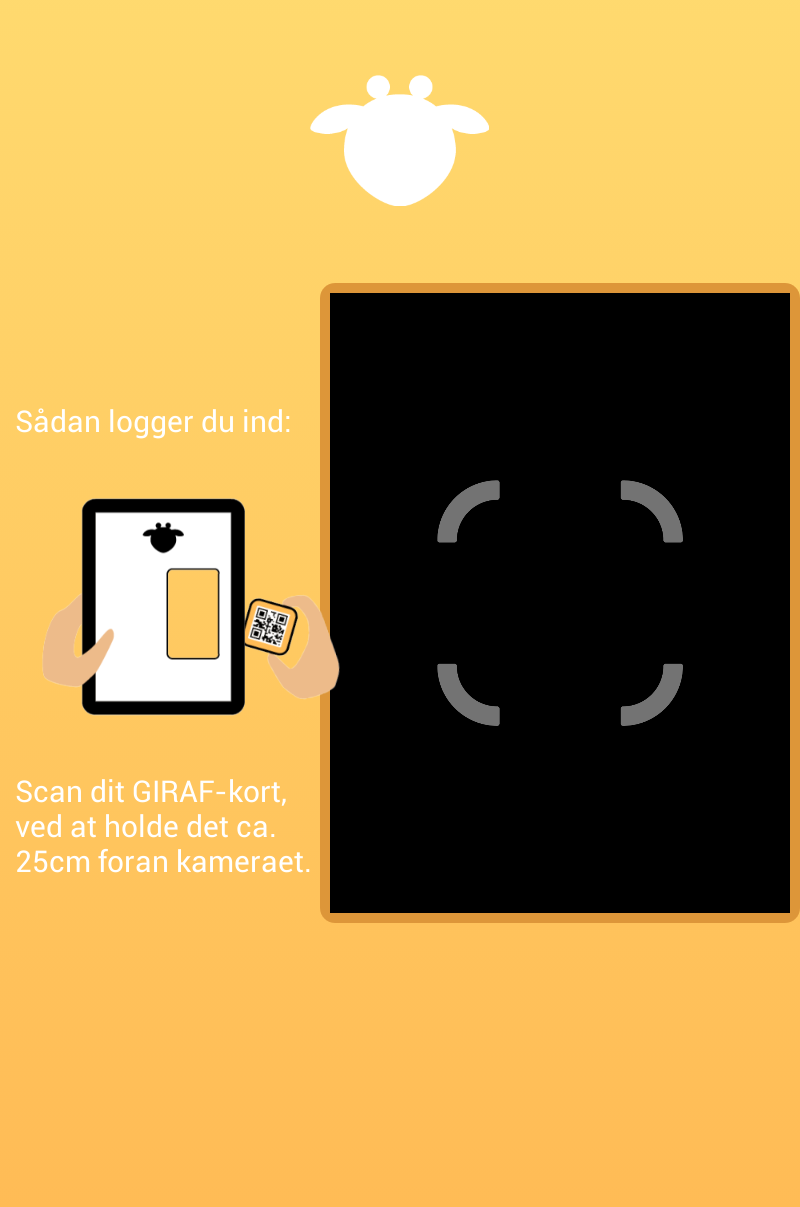
\includegraphics[width=\textwidth, height=3in, keepaspectratio=true] {screenshots-old-giraf/giraf-authenticationactivity.png}
	\caption{\textit{Authentication} activity.}
	\label{fig:launcheractivity:auth}
	\end{subfigure}
	
	\quad % Inserts extra space between rows of subfigures
	
	\begin{subfigure}[b]{.48\textwidth}
	\centering
	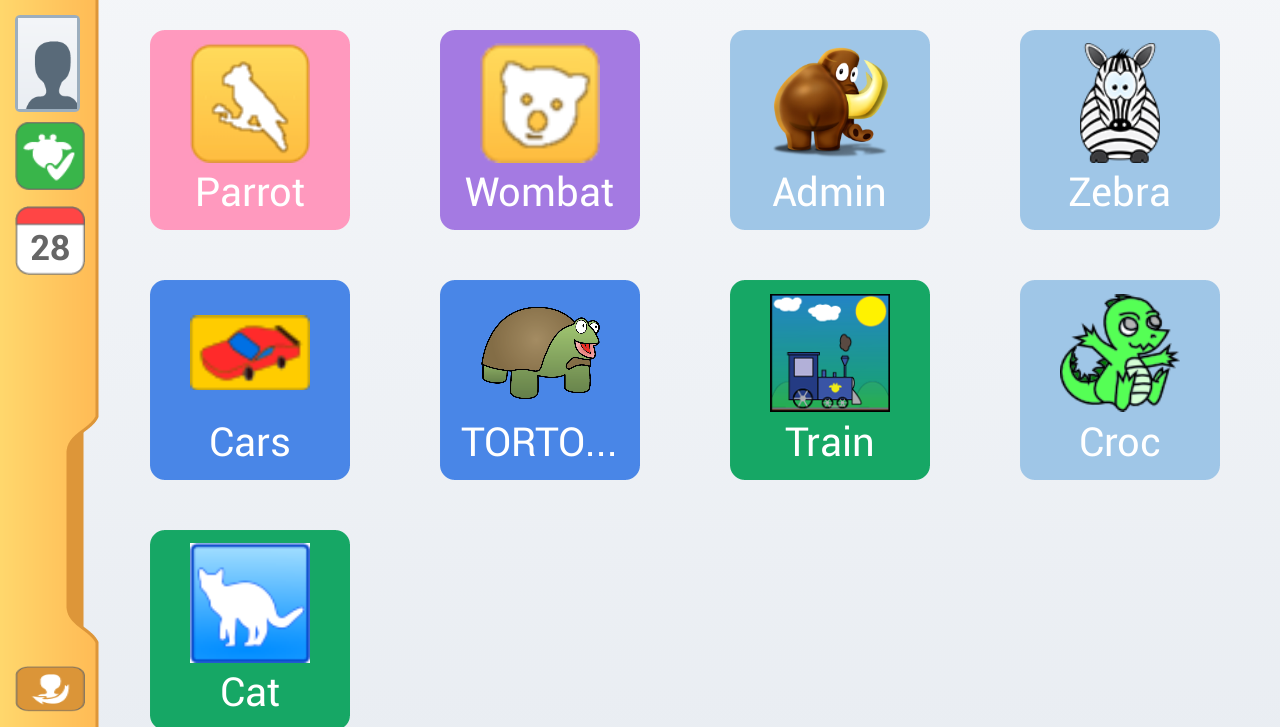
\includegraphics[width=\textwidth]{screenshots-old-giraf/giraf-homeactivity.png}
	\caption{\textit{Home} activity.}
	\label{fig:launcheractivity:home}
	\end{subfigure}
	\begin{subfigure}[b]{.48\textwidth}
	\centering
	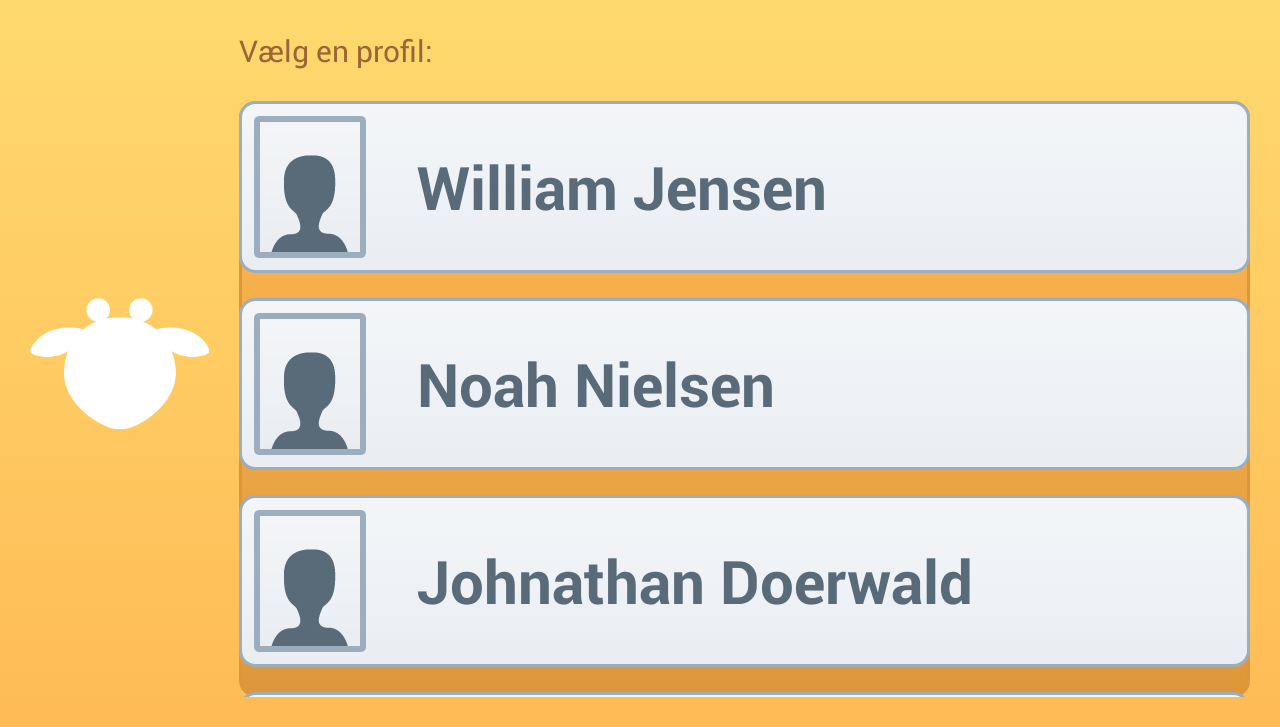
\includegraphics[width=\textwidth]{screenshots-old-giraf/giraf-profileselect.png}
	\caption{\textit{ProfileSelect} activity.}
	\label{fig:launcheractivity:profile}
	\end{subfigure}
\caption{Activities of the \giraf application.}
\label{fig:launcheractivities}
\end{figure}

\paragraph{Logo activity} is not responsible for anything else than showing the \giraf logo for a specified amount of time (as seen in \cref{fig:launcheractivity:logo}), and then redirecting the users to the proper activity.
It redirects to Authentication activity if the user is not logged in, or to the Home activity if the user is already logged in.\thilemann{Discuss if fx activities should be written as inline listings.}

\paragraph{Authentication activity} requires the user to authenticate him- or herself before proceeding. 
\citet{launcher2012} describes how user identification is necessary, as the \giraf settings must be able to vary from user to user. 
The report furthermore describes how autistic children might have problems using a traditional user-name and password system. 
Therefore, the authentication activity is based on a QR-scanner, as seen in \cref{fig:launcheractivity:auth}.
Each child and guardian then uses a small brick with their personal QR-code they scan to identify themselves. 
The activity loads the user information from the database, and proceeds to the Home activity.

\paragraph{Home activity} allows the user to launch \giraf applications available to his or hers user account. 
The availability of an applications depends on whether the application exists locally on that device, and on whether the user is marked in the database as having proper access rights to that application.
The \textit{Home} activity for a test guardian user is seen in \cref{fig:launcheractivity:home} with the user's installed \giraf applicatons.
Furthermore, a number of widgets allows the user to see the synchronization status of the local database in relation to the remote database, and a widget showing current date. 
There is also a button that allows the user to log out, and return to the Authentication activity.
Finally, there is a colour palette hidden in a drawer component, where the user can change the base colour of each installed applications. 
The idea is to make it easier for the children to differentiate between the various applications by being choosing their own colourscheme. 
Ideally the choice of colour should also reflect in the application started from the \launcher, giving the child consistent visual associations throughout \giraf.
The latter is for example implemented in the \textit{Timer} application.\vagner{Add a source to this}\thilemann{Is that necessary?}

\paragraph{Profile Select activity} is started when a guardian launches an application from \launcher. 
It displays a list of all children associated with this guardian (as seen in \cref{fig:launcheractivity:profile}), allowing him or her to choose which child's profile to use when launching the selected application. 
When a child is selected, the application launches, omitting the \textit{Profile Select activity}.
\subsection{Drawer}\label{sec:launcher:drawer}
The drawer is a separate view that is situated in the left-hand side of the \textit{Home} activity.
Its main purpose is to allow \launcher users to apply a new colour-scheme to their installed \giraf applications.

The concept of the drawer is a component that can be shown and hidden at will.
This means that only part of the drawer is visible at all time; it can be dragged towards the centre of the screen to reveal its contents.
Apart from enabling the users to switch colours of their installed \giraf applications, it also contains various informative widgets.
These widgets are a calendar, implemented as \lstinline{GWidgetCalendar}, a server connection indicator, implemented as \lstinline{GWidgetConnectivity}, and a logout button, implemented as \lstinline{GWidgetLogout}.
The implementations of these widgets are a part of \lstinline{GirafComponents}, a separate project in the \giraf system that handles customized Graphical User Interface components.
It should be utilized throughout all \giraf applications to make them look and feel the same.

Illustrations of the drawer in closed and opened positions can be seen in \cref{fig:drawerclosed,fig:draweropened} respectively.

\begin{figure}[h] % Billeder af draweren i åben og lukket tilstand
\centering
	\begin{subfigure}[b]{.48\textwidth}
	\centering
	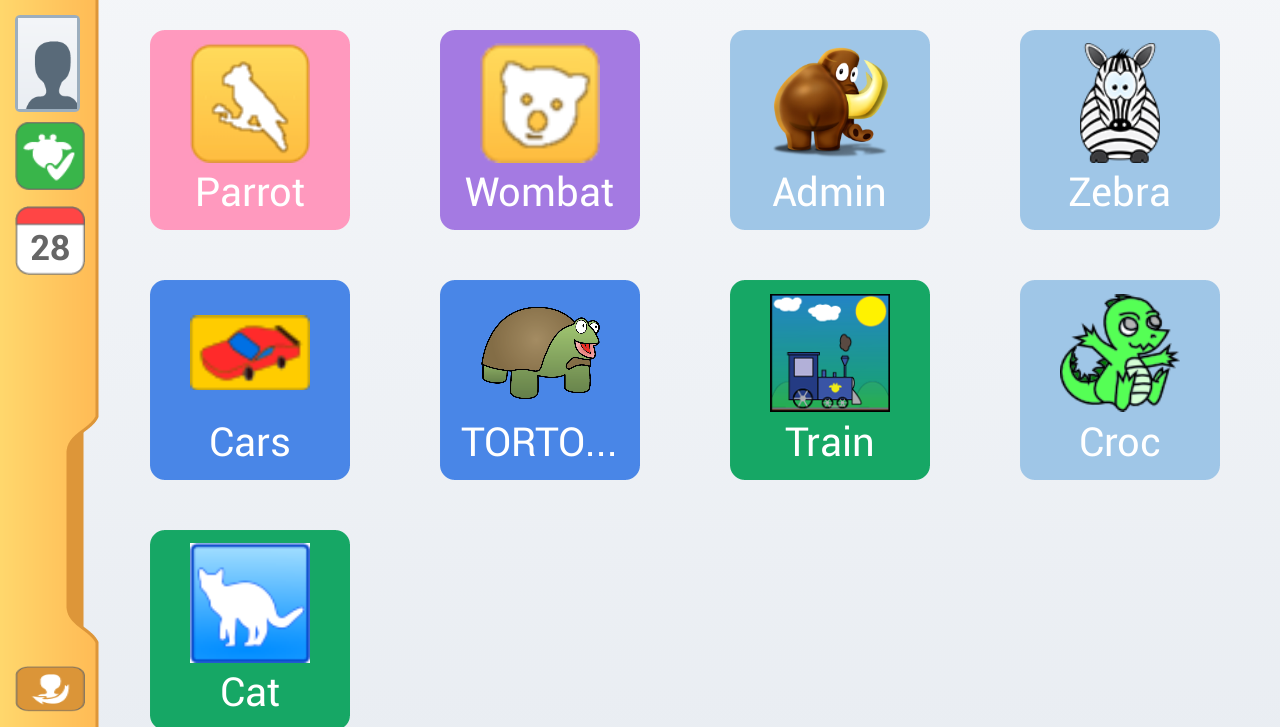
\includegraphics[width=\textwidth]{screenshots-old-giraf/giraf-homeactivity.png}
	\caption{Drawer closed.}
	\label{fig:drawerclosed}
	\end{subfigure}
	\hfill
	\begin{subfigure}[b]{.48\textwidth}
	\centering
	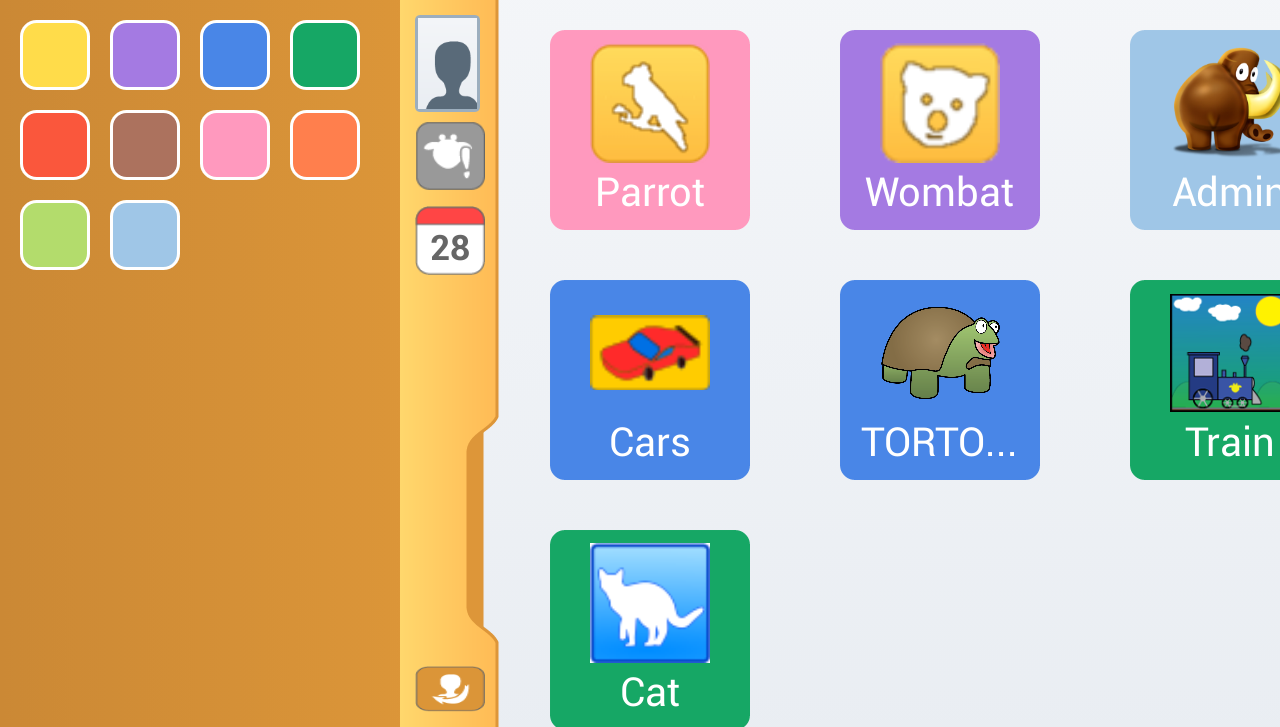
\includegraphics[width=\textwidth]{screenshots-old-giraf/giraf-drawer-fullyextended.png}
	\caption{Drawer fully extended.}
	\label{fig:draweropened}
	\end{subfigure}
\caption{States of the drawer component shown on \textit{Home} activity.}
\label{fig:drawerstates}
\end{figure}

As indicated by \cref{fig:drawerstates}, the drawer already meet the requirement that a colour can be dragged onto an application.
In spite of this, many deficiencies have been located, which are further enlightened by the following sections.

\subsubsection{The Original Drawer}

The original drawer would open by pressing and holding the bar and sliding it to the right.
While being opened, the drawer would push the application icons along with it to the right, resulting in some icons disappearing off-screen to the right.
Furthermore, the drawer would stop when pressure was released from the touch-screen, meaning it could be left in a half-open, half-closed state.
To change the colour of an application, a colour could be drag-and-dropped onto an icon. 
The result would be immediately apparent, as the colour framing the icon would change to the selected colour.

\subsubsection{Desired Improvements}

Since no formal requirements are available and the project group had yet to have a meeting with the customer, the suggested improvements below is based on what we find to be natural requirements of such a User Interface component. 

\begin{itemize}
\item The drawer should be either open or closed. A half-open or half-closed state should result in the drawer popping into the state closest to its current position.
\item The drawer should close while a colour was being dragged, and open again when dropped.
\item The drawer should not push the application icons out of the screen.
\item The source code responsible for the animation of the drawer and the layout of \lstinline{HomeActivity} should be refactored in order to:
\begin{itemize}
\item take advantage of standard Android animations and layout features,
\item allow the activity to dynamically adjust according to display size and
\item reduce the amount of clutter in the source code and improve readability.
\end{itemize}
\end{itemize}

The implementation of the improvements is described in \cref{sec:developments:drawerimprovements}.

\section{Developments}\label{sec:sprint1:developments}
This section considers the problems found in the Analysis and Design (\cref{sec:sprint1:analysis}) of the first sprint.
\vagner{Mention minor bugs, debug mode and focus on home activity, drawer, and restructuring of layout. Also mention functional tests somehow... bare skriv en lille intro}
\subsection{Minor Bugs}

Several minor bugs, anomalies and things that did not work as expected were found in the beginning of the spring.
Considering their negligible significance, we will not discuss them in depth, but rather describe each briefly.

\subsubsection{Child Mode}
Regardless of whether the currently logged in profile is a child or a guardian, \launcher opens the \lstinline{ProfileSelector} before opening an application.
It should only open that activity while using a logged in guardian profile.
The issue is solved by checking on the \lstinline{getRole()} parameter of a profile and then appropriately override the \lstinline{OnClickListener} of the profile selector dialog, depending on the role. 

\subsubsection{Force Landscape Mode}
It is clear from reading previous reports describing \launcher that landscape mode should be forced in all \giraf applications.
Since \launcher is the only application able to enter portrait mode, it is corrected by changing \lstinline{AndroidManifest.xml} to only allow landscape mode for all activities, which contains essential information that is used by the Android system to control its behavior\cite{appManifest}.

\subsubsection{Issues related to other groups}
Two issues caused by other projects are also discovered:

\begin{itemize}
\item The \lstinline{GButton} widget from \textit{GIRAF Components} library crashes any activity that implements it.
\item Danish characters are not encoded correctly in the database.
\end{itemize}

The issues are reported to the groups responsible for these components through our issue tracker, which in effects handles their responsibility over to the other groups.
\thilemann{Write about the improvements of the launcher}
\thilemann{Maybe also something about refactoring the xml files}
\subsection{Drawer Improvements}\label{sec:developments:drawerimprovements}
As mentioned in \cref{sec:launcher:drawer}, the drawer was opened by pressing and dragging the drawer border.
The code working this animation was based on an \lstinline{OnTouchListener}, focusing mainly on the \lstinline{MotionEvent.ACTION_MOVE} event.
\lstinline{MotionEvent.ACTION_MOVE} would set the position of the entire drawer, panel and bar, to the exact point it had currently been moved to and redraw the elements.
Because the \lstinline{ScrollView} containing the application icons was set to \lstinline{android:layout_toRightOf} in the layout XML files, the \lstinline{ScrollView} would adjust itself to the new position each time the event fired.

The panel of colours was implemented using a \lstinline{GridView} - using the command \lstinline{AppColors.setAdapter(new GColorAdapter(this));}, the \lstinline{GColourAdapter} from \lstinline{OasisLib} would create the correct panel.

Selecting a colour and assigning it to an application worked by means of an \lstinline{OnDragListener} called \lstinline{GAppDragger}.

\subsubsection*{The Improved Drawer}

Opening and closing the improved drawer was implemented with an \lstinline{OnTouchListener} through the \lstinline{MotionEvent.ACTION_DOWN} event and a standard Android \lstinline{TranslateAnimation}.
Pressing the bar fires the event and begins the animation.
A \lstinline{boolean} variable determines whether the drawer was open or closed when the event fired and thus if the animation should translate left or right.
By also adding an \lstinline{OnDragListener} to the drawer, the animation would also play when dragging and dropping colours from the panel; closing the drawer on \lstinline{DragEvent.ACTION_DRAG_STARTED} and opening it again on \lstinline{DragEvent.ACTION_DRAG_ENDED}.

Having the \lstinline{ScrollView} containing the application icons remain static during the animation, was solved by reorganising the source code responsible for the user interface layout. 
Previously, all elements were merely declared in the XML layout file, while positioning of the elements was statically set in the \lstinline{HomeActivity} load code - over 100 lines of parameter setting code.\vagner{maybe not include mocking the previous group?}
This was refactored to have the all positioning declared dynamically depending on screen size, apart from the positioning of the \lstinline{ScrollView}.\vagner{Stefan, write intelligent stuff about dynamic positioning of the ScrollView}
\vagner{Add documentation about the icon indicating opening and closing of the drawer}

The improved drawer fulfils all desired the previously specified requirements, and provides a smoother and more pleasant experience for the user, while refactoring of the acting code provides clarity and readability of developers.\jesper{Is this a little arrogant, considering we haven't actually shown it to users?}\vagner{True, and in sprint 2 we learn that the user doesnt even need the drawer. However, this was what we thought was requirements at the time of writing.}


\subsection{Authentication Activity Error}
When starting \launcher for the first time, the application crashed and threw an \lstinline{OutOfMemoryError} when reaching the \authenticationactivity.
The core of this problem is caused by an animation in the activity, implemented as an instance of the Android class \lstinline{AnimationDrawable} -- a class designed to create animations from a sequence of images.
According to the Android documentation \citet{androidreference}, the implementation is technically correct, but it is found that when an instance of \lstinline{AnimationDrawable} is created, it loads the entire sequence of images into main memory of the device at once.
The images are contained within the application in the compressed Portable Network Graphics (PNG) format.
However, as they are loaded, Android converts each image to a 32-bit bitmap, which is 4 bytes per pixel, making the images take up about 20 times the space, thus resulting in the animation using about 40 MB of memory. 
We hypothesized that this was the source of the \lstinline{OutOfMemoryError}.

One solution to this problem is to create a new class which simulates the behaviour of \lstinline{AnimationDrawable}.

By simulating \lstinline{AnimationDrawable}, we only keep one image in memory at all times and avoid the error.
This is achieved by a recursive method, which is changing the shown image automatically.
The images are stored in a static array which is iterated repeatedly using the method \lstinline|postDelayed()| which is possible to run code after a set amount of time.

\begin{lstlisting}[caption={Improved implementation of handling the animation.},label={lst:methodPlay}]
private void play(final int pFrameNo){
  mImageView.postDelayed(new Runnable(){
    @Override
    public void run() {                    
      mImageView.setImageResource(mFrames[pFrameNo]);

      if(pFrameNo == mLastFrameNo)
        play(0);
      else
        play(pFrameNo + 1);
    }
  }, mDuration);
}        
\end{lstlisting}
As one of our goals is to increase the reliability of \launcher, we decided to conduct functional testing on the application.
We studied the specifications formulated by the earlier development teams in \citet{launcher2011,launcher2012}, and then studied how well \launcher correspond to these specifications, by using the program in a number of different ways. 

Furthermore, a number of test cases are not directly derived from the old specifications, but from what we find reasonable to expect of the application, based on our own knowledge of the system.

The tests described here are performed by operating the running application, and are explicitly not based on our knowledge of the source code. 
This characterizes our tests as being dynamic black box testing. 

A number of test cases that would have been relevant, is not performed in this sprint as we deem that they not sufficiently interesting, considering the time needed to run them. This includes using \launcher with a varying set of applications and children.
These test cases require significant changes to the test data hard coded into the \giraf system, or repeatedly installing and uninstalling applications from the device.
As there is currently no central repository of stable application builds, most of the time would be spent building, installing and resetting different applications.

We only describe the results we find the most interesting in this section; mainly tests that failed in a significant way.

\subsection{Specifications}
In the 2011 report by \citet{launcher2011}, the following specification for \launcher is presented:

\begin{quote}
\begin{itemize}
	\item \textit{List only applications that is part of the \giraf system.}
	\item \textit{List only applications that the user is able to use, according to the user's capabilities.}
	\item \textit{List only applications if their usage is not limited by the current location or time.}
	\item \textit{Only display application names if the user is able to read.}
\end{itemize}
\end{quote}

Common to all these, is that they are either difficult to test, or simply not implemented (some may have been to some degree in 2011, but then removed by the 2012 team).
The difficulty stems from the necessity of manipulating test data, that is hard coded into the local database of each device. 
We decided it would be more reasonable to revisit these test cases when \giraf's database system is ready for use.

The 2012 report by \citet{launcher2012} contains no explicit specifications, but does contain a list of use cases. 
These form the basis of our tests:

\begin{quote}
\begin{itemize}
	\item \textit{New guardian log in.}
	\item \textit{Configuring an application for a child.}
	\item \textit{Launching an application for a child in guardian mode.}
	\item \textit{Letting a child use an application for a limited time.}
\end{itemize}
\end{quote}

Note that their report also contains an explanation of each use case. 
We leave these out for brevity.

\subsection{Test Results}\label{sec:sprint1:testing_results}
Below is shown a selection of our test cases and their results.
As mentioned in the introduction of this section, we will only discuss the most interesting results, i.e. tests that led to the discovery of significant issues.

\subsubsection{Changing the Colour of an Application Icon}

\paragraph{Specification:} Configuring an application for a citizen.
\paragraph{Test case:} Use the drawer to change the colour of an application, and check if the change is applied to both the application's icon, and its own user interface.
\paragraph{Result:} The colour of the icon changed immediately, but when starting the application, it still used the pre-change colour. 
A little experimenting showed that the change is not applied to the application until the user logs into \launcher again.
\paragraph{Resolution:} The issue was resolved, and the change in colour is now reflected in the application immediately.

\subsubsection{Applications that Crash Launcher}

\paragraph{Specification:} Starting an application for a citizen in guardian mode.
\paragraph{Test case:} Open an application with a randomly selected citizen profile by using the profile selector.
\paragraph{Result:} While not directly related to the intent of the use case, during the test, we attempted to open what turned out to be a non-working version of a \giraf application. 
The application suffered from an unhandled exception, causing both it and \launcher to crash. 
This is not satisfactory, as \launcher should always work on top of the device operating system, denying the citizen access to device settings when using the device without supervision.
\paragraph{Resolution:} The issue was resolved by making \launcher catch all exceptions thrown by the \giraf applications it hosts.

\subsubsection{Use of Device Buttons}

\paragraph{Specification:} The device buttons (\textit{Back}, \textit{Home}, and \textit{Multitasking}) should have no effect in \mainactivity and \authenticationactivity, as the user should not be able to ``back out'' of \launcher to the device OS.
\paragraph{Test case:} Use the device buttons in different activities and situations.
\paragraph{Result:} In both \mainactivity and \authenticationactivity, applying the \textit{Home} and \textit{Back} buttons made \launcher restart. 
The \textit{Multitasking} button always activates the multitasking screen of the device OS.
\paragraph{Resolution:} The \textit{Back} button are suppressed by overriding a listener method.
We were unable to find similar means for suppressing the other two buttons, as we unsuccessfully returned to this issue in the second sprint, as described in \cref{sec:sprint2:backlog}.

\section{Sprint End}\label{sec:sprint1:review}
\subsection{Evaluation}
Overall, the first sprint was a success for us.
All task were finished and \launcher is now ready for the sprint review together with the clients, receiving feedback regarding the next steps.

However, for various reasons, the meeting does not yield the desired results for planning the next sprint.
Therefore, the groups decide to appoint a single person responsible for planning and executing this meeting in the future.
The chosen person is from this group, so the details of this and later sprint reviews are discussed in depth in \cref{sec:collab:sprintend}.

\subsection{Backlog}
As mentioned above we did not get any feedback during the sprint review to use for planning our next sprint.
We still think there are elements to improve in \launcher, but we cannot immediately continue the development, before having explored whether the clients have further requirements for the application.
These are explored in \cref{sec:sprint2:overview}.